\documentclass[12pt]{niuthesis}
% \documentclass[12pt,singlespacing]{niuthesis}

% some packages are loaded here
\usepackage{latexsym}		% to get LASY symbols
\usepackage{graphicx}		% to insert PostScript figures
\usepackage{rotating}           % defines sidways table and figure env.
\usepackage{amsmath}
% \usepackage{hyperref}		% to insert hyperrefs

%%%%%%%%%%%%%%%%%%%%%%%%%%%%%%%%%%%%%%%%%%%%%%%%%%%%%%%%%%%%%%%%
% Some LaTeX macros

\newcommand{\twochoices}[2]{\left\{ \begin{array}{lcc}
        \displaystyle #1 \\ \vspace{-10pt} \\
        \displaystyle #2 \end{array} \right. } %}

\newcommand{\twovec}[2]{\left(\begin{array}{c} #1 \\ #2 \end{array}\right)}

\newcommand{\twomatrix}[4]{\left(\begin{array}{cc} #1 & #2 \\ 
     #3 & #4 \end{array}\right)}

% Uncomment the following line for a List of Symbols
% \newcommand{\listofXXX}{\chapter*{List of Symbols}
\addcontentsline{toc}{chapter}{List of Symbols}

\begin{tabular}{cp{0.6\textwidth}}
  $x$ & position \\
  $v$ & velocity \\
  $a$ & acceleration \\
  $t$ & time \\
  $F$ & force
\end{tabular}\\
and many more!

\chapter*{List of Rockets}
\addcontentsline{toc}{chapter}{List of Rockets}

\begin{tabular}{cp{0.6\textwidth}}
  1232 & some old chinese rocekts \\
  1792 & rocket build by Hyder Ali \\
  1957 & R-7 (launched sputnik) \\
  1967 & Saturn V
\end{tabular}\\
and many more!

%%%%%%%%%%%%%%%%%%%%%%%%%%%%%%%%%%%%%%%%%%%%%%%%%%%%%%%%%%%%%%%%%%

%%% Local Variables: 
%%% TeX-master: "mythesis"
%%% End: 
}

%%%%%%%%%%%%%%%%%%%%%%%%%%%%%%%%%%%%%%%%%%%%%%%%%%%%%%%%%%%%%%%%%%
% Choose the chapter(s) / files you want to work with

%%% use this to compile all chapters
\def\files{ch1,ch2,ch3,refs,app1,app2}

%%% use this to work with only one chapter
% \def\files{ch2}

\includeonly{\files}

%%%%%%%%%%%%%%%%%%%%%%%%%%%%%%%%%%%%%%%%%%%%%%%%%%%%%%%%%%%%%%%%%
\begin{document}

\title{Magnetometer-less State-Estimation \\ of a Unicycle Model Mobile
Robot \\ using a Cascaded Kalman Filter Framework}

\author{Tommy Le}

\major{Mechanical Engineering}
\degree{Thesis}{M.S.}{Masters of Science}
\degreedate{Dec}{2023}
\department{Department of Mechanical Engineering}
\director{Dr. Ji-Chul Ryu}

\begin{abstract}

\end{abstract}

\begin{acknowledgments}
  Here's where you acknowledge folks who helped.

\end{acknowledgments}

\begin{dedication}
  To all of the fluffy kitties.

\end{dedication}

% comment this to suppress prologue
\MakeThesisPrologue % includes table of contents
% \tableofcontents

\chapter{Introduction}		% chapter 1
\label{introchap}		% for reference (\ref{introchap})

This section will cover background information on mobile robot kinematic models,
IMU state estimation, Kalman Filtering methods, and cascading KF framework. 


\section{Motivation}

Talk about the development of miniature robots. Talk about our spherical robot design.
The small size of the robot makes it difficult to use a magnetometer due to the close
proximity of the motors and sensors. Using an external sensor is clunky or not
realistic. 

\section{Literature Review}

This section should go over the papers I have gone over. This includes 
Song 2018 on the cascaded KF framework, as well as other papers using external 
sensors to get more robust heading. 

\section{Objective}

To tackle these challenges, this thesis aims to find a novel way to estimate
a mobile robots states using only a 6DOF IMU with a unicycle model wheeled mobile 
robot. The thesis will have an algorithm with only a 6DOF IMU as well as having the
option to add an additional sensor to provide more robust localization.

%%%%%%%%%%%%%%%%%%%%%%%%%%%%%%%%%%%%%%%%%%%%%%%%%%%%%%%%%%%%%%%%%%

%%% Local Variables: 
%%% TeX-master: "mythesis"
%%% End: 
		% file with Chapter 1 contents
\chapter{Methods}
\label{mathchapter}

This part will be an overview of the overall framework of the algorithm. It
will first discuss preprocessing methods. These methods involve NMNI, NDZTA,
and error compensation in the gyroscope and accelerometer. Afterwards it will 
discuss the first and second kalman filter models, then the optional block
containing the additional sensor to improve the performance of the filter.

%%% IMU Section

\section{IMU Preprocessing}

Here I will first talk about what an IMU is, 6DOF vs. 9DOF, how each sensor
works, and the inherent errors in each sensor. 

It will then cover the planned signal processing methods for each sensor on the 
IMU and go in depth about each algorithms implementation.

\subsection{Accelerometer Signal Processing}

This subsection talks about the preprocessing methods that will take place on
the accelerometer data coming from the IMU as well as the numerical integration 
methods used for displacement calculation.

\subsubsection{Displacement Measurement from Acceleration Data}

Euler integration, trapezoidal, RK4. (Better integration = better data) 
Don't think I really need to explain this right now.

\subsubsection{No Displacement Zero Translational Accumulation (NDZTA)}

\emph{Sci-hub Link: https://sci-hub.live/https://ieeexplore.ieee.org/
document/9268038 \\ }

Removing the noise in accelerometer data during stationary points in time is 
done by finding a way to have the system understand when it is stationary. The 
No Displacement Zero Translation Accumulation (NDZTA) algorithm accounts for 
this by calculating a threshold value that indicates whether the system is in 
motion or not. Figure 2.1 illustrates the logic of the algorithm.

\begin{figure}[h]
  \centerline{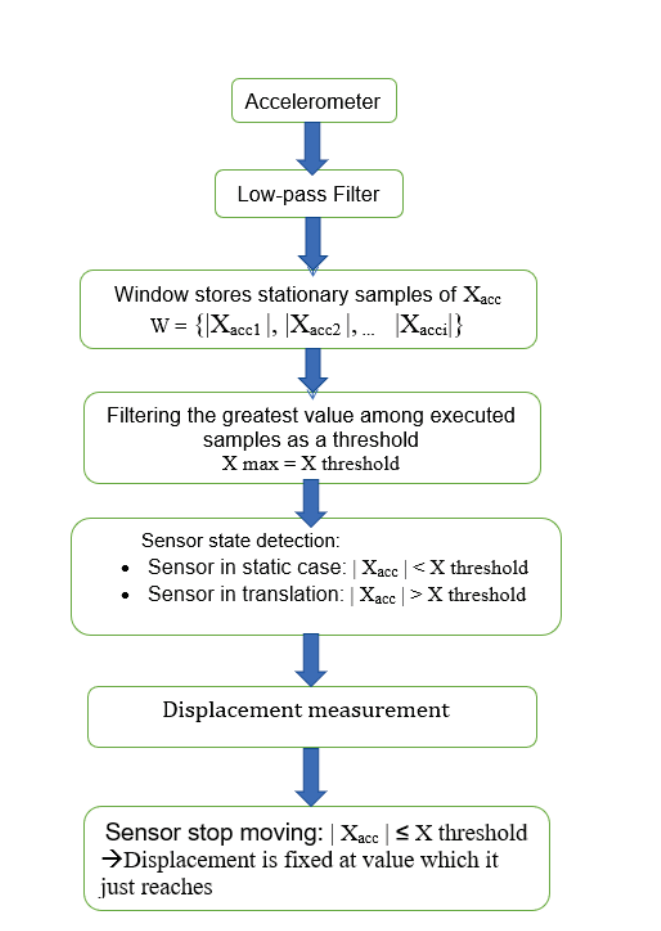
\includegraphics[height=95mm]{temp_NDZTA.PNG}}
  \caption[NDZTA Flow]{
    NDZTA flow
    }
  \label{fig:NDZTA}
\end{figure}

First a low pass filter is applied to the accelerometer data to eliminate
the inherent high frequency noise. After the filter is applied, a maximum
value is collected from a sampling window during an initial static position. 
This maximum value becomes the threshold that helps the system realize it 
is not in motion. Now the displacement is calculated based on this found 
threshold which signifies the boundary between static and dynamic motions. 
The algorithm works by comparing the real-time acceleration data $a$ with 
the threshold $a_{th}$ to decide if displacement calculation is needed. This 
comparison is demonstrated in equations 2.1 and 2.2.

\begin{equation}
	a > a_{th}, \textnormal{ Sensor is in motion. Carryout displacement calculation \\}
\end{equation}

\begin{equation}
  a \le a_{th}, \textnormal{ Sensor is static. Set acc = vel = pos = 0 \\}
\end{equation}


Note that the displacement calculation has many errors due to noise in 
the sensor signals and numerical integration causing the error to grow. In 
order to eliminate the error, the NDZTA algorithm proposes a method composed
of these 3 main steps.

\emph{ \\ Step 1: Threshold Calculation \\
 Step 2: Motion Detection \\ 
 Step 3: Displacement Measurement \\ }

During each detection of the static case, the threshold value is updated 
depending on equation 2.3.

\emph{\\ Equation 2.3 here! \\}
some conditional statement that I cannot remember.

\subsection{Gyroscope Signal Processing}

This subsection talks about the preprocessing methods that will take place on
the gyroscope data coming from the IMU.

\subsubsection{Bias Compensation}

Don't think I need to really explain this right now.

\subsubsection{No Motion No Integration (NMNI)}

\emph{Sci-hub link: https://sci-hub.live/https://ieeexplore.
ieee.org/document/9247295 \\https://sci-hub.live/https://www.sciencedirect.
com/science/article/abs/pii/S0924424721001540 \\ }

To find roll, pitch, and yaw angles, the angular rate data from the gyroscope
is numerically integrated. Due to multiple different error sources, noise 
and drift problems will cause the gyroscope data to vary. 

To compensate for these errors, the No Motion No Integration (NMNI) algorithm 
is used. This algorithm only allows numerical integration when dynamic motion
is detected. Similar to the NDZTA algorithm discussed in previous sections, 
this algorithm finds the maximum value within sampled data during an initial 
window of static motion. This max value is set as a threshold value, and 
the real-time data collected by the gyroscope is compared with the threshold 
value to determine if the system is in static or dynamic motion. The overall 
logic of the algorithm can be seen in figure 2.2 below.

\begin{figure}
  \centerline{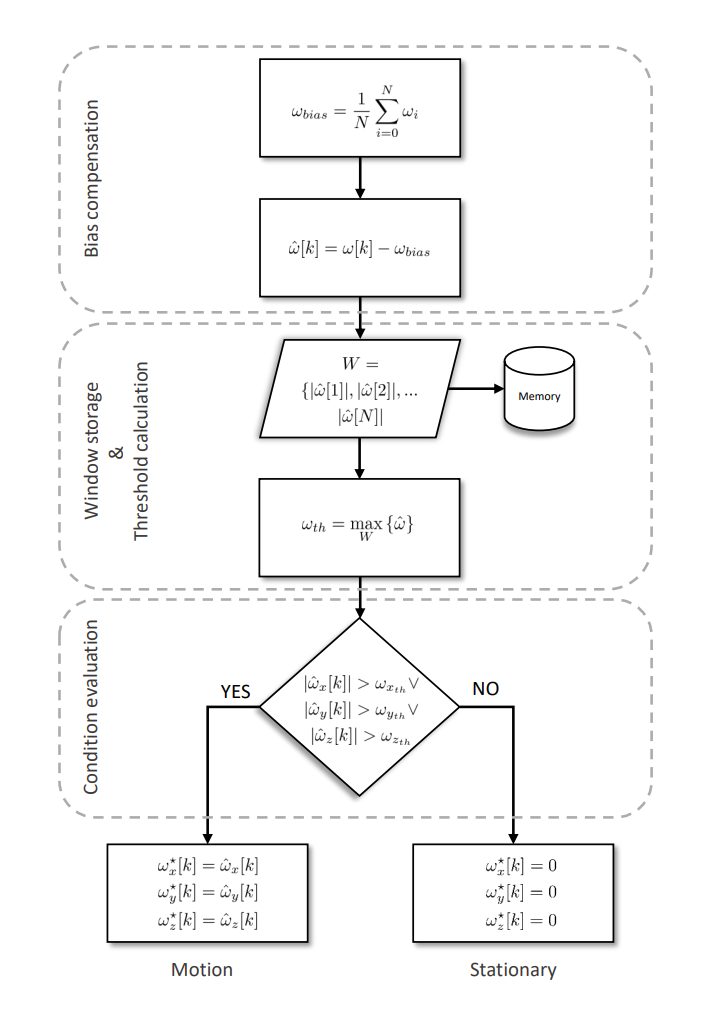
\includegraphics[height=95mm]{temp_NMNI.PNG}}
  \caption[NMNI Flow]{
    NMNI flow
    }
  \label{fig:NMNI}
\end{figure}

Maybe enter equations here too. But seems redundant.

%%%
%%% First KF block
%%%

\section{First KF: Course Correction Extended Kalman Filter}

This section covers the first Kalman Filter in the cascaded Kalman Filter framework.
This Kalman Filter uses the unicycle kinematic model as the process model, and gets
bias compensated feedback position data from the accelerometer as the measurement 
model. 

\subsection{Process Model}

Kinematic model follows the common unicycle model for wheeled-mobile robots (WMRs).
This thesis is assuming 2D planar motion so the states are x, y, and theta.
\\ \\
\begin{equation}
  x = z = [x, y, \theta]^T
\end{equation}

\begin{equation}
  f = \begin{bmatrix}
        vcos(\theta) & 0 \\
        vsin(\theta) & 0 \\
              0      & w
      \end{bmatrix}
\end{equation}
where $v$ and $w$ are the linear and angular velocity of the mobile robot.

\begin{equation}
  F = \begin{bmatrix}
    1 & 0 & -vsin(\theta) \\
    0 & 1 &  vcos(\theta) \\
    0 & 0 &       1
  \end{bmatrix}
\end{equation}



\subsection{Measurement Model}

The measurement model here is identity because the states can be directly 
accessed with minimal calculations. Going into this system will be the corrected 
and compensated position and orientation data that is found from our second KF.
These are then used to estimate the states taking into account the robots kinematic
constraints along with the sensor measurements.  

\emph{Add equations on how pose is found using sensor data}

\begin{equation}
  h = \begin{bmatrix}
    1 & 0 &  0 \\
    0 & 1 &  0 \\
    0 & 0 &  1
  \end{bmatrix}
\end{equation}

\begin{equation}
  H = \begin{bmatrix}
    1 & 0 & 0 \\
    0 & 1 & 0 \\
    0 & 0 & 1
  \end{bmatrix}
\end{equation}

%%%
%%% Second KF block
%%%

\section{Second KF: Bias Estimation Kalman Filter}

This section covers the second Kalman Filter in the cascaded Kalman Filter 
framework.This Kalman filter uses the gyroscope model as the process model, 
and uses the accelerometer data as the measurement model to estimate our 
states as well as correction terms to compensate for sensor errors.

\subsection{Process Model}

This states are orientation error ($\delta\phi$), velocity error ($\delta v$), 
gyroscope bias ($b_g$), and accelerometer bias ($b_a$).

\begin{equation}
  \boldsymbol{x}_2 = [\delta\boldsymbol{\phi}^T, \delta\boldsymbol{v}^T,
       \boldsymbol{b}^T_g, \boldsymbol{b}^T_a]^T
\end{equation}


\begin{equation}
  f = \begin{bmatrix}
        \boldsymbol{0}_{3x3} & \boldsymbol{0}_{3x3} & \boldsymbol{-C}^n_b & \boldsymbol{0}_{3x3} \\
        \boldsymbol{S} & \boldsymbol{0}_{3x3} & \boldsymbol{0}_{3x3} & \boldsymbol{C}^n_b \\
        \boldsymbol{0}_{3x3} & \boldsymbol{0}_{3x3} & -\beta_g\boldsymbol{I}_{3x3} & \boldsymbol{0}_{3x3} \\
        \boldsymbol{0}_{3x3} & \boldsymbol{0}_{3x3} & \boldsymbol{0}_{3x3} & -\beta_a\boldsymbol{I}_{3x3}
      \end{bmatrix}
\end{equation}

C (don't know if definition is correct) is a rotation matrix. S is a skew symmetric matrix of acceleration representing
vector cross product. $\beta$ are the Markov process time constants that model our
biases. 

\begin{equation}
  \boldsymbol{C}^n_b = \begin{bmatrix}
        cos(\phi_D) & -sin(\phi_D) & 0 \\
        sin(\phi_D) &  cos(\phi_D) & 0 \\
        0 & 0 & 1 \\
      \end{bmatrix}
\end{equation}

\begin{equation}
  S = \begin{bmatrix}
        0 & -a_D & a_E \\
        a_D & 0 & -a_N \\
        -a_E & a_N & 0 \\
      \end{bmatrix}
\end{equation}

\subsection{Measurement Model}

Measurements are course angle error and velocity measurements. Course angle error
is found by taking the difference between the KF estimated heading angle from the 
gyro and unicycle model and the estimated heading found from using the previous 
and current position data that provides the heading for the robot to linearly 
move from the previous point to the current point.

\begin{equation}
  \delta\theta = \theta_{est} - \theta_{acc}
\end{equation}

where $\theta_{est}$ is the heading estimated by the kalman filter and $\theta_{acc}$ 
is the heading found from the position data. 

\emph{COMMENT} \\
But doesn't heading from kinematics come from acc and gyro already? So instead,
take the improved heading from fusing kinematics with acc and gyro, and pass to 
gyro KF instead of heading error. 

So first KF takes x, y, $\theta$ as measurement and outputs $\theta$ into KF2. 
KF2 then takes in v and $\theta$ to estimate errors to correct/compensate 
sensor measurements and vel and orientation errors. These improvements of 
measurement errors and state errors should improve x, y, $\theta$ and improve 
estimates in the first KF. Those will be the states that we care more about.

But if we are just going to use the states estimated by the first KF, why don't 
we just find orientations and pass it to first KF rather than find errors, then 
externally correct them then pass them to the first KF. 
\\
\emph{COMMENT}

\begin{equation}
  z_2 = [\delta\theta, \boldsymbol{v}]^T
\end{equation}

\begin{equation}
  h = \begin{bmatrix}
      \begin{bmatrix}tan(\phi_N)cos(\phi_D) & tan(\phi_N)sin(\phi_D) & -1\end{bmatrix} & \boldsymbol{0}_{1x3} & \boldsymbol{0}_{1x3} & \boldsymbol{0}_{1x3} \\
      \boldsymbol{0}_{3x3} & \boldsymbol{I}_{3x3} & \boldsymbol{0}_{3x3} & \boldsymbol{0}_{3x3}
      \end{bmatrix}
\end{equation}

\section{Estimation with Additional Sensor}

This sensor should be one that can give position data. GPS, camera, encoder.
From this extra sensor, you can set up a cost function that models the error 
in the measurements and minimize it using gradient descent or something to 
hopefully get the best estimate in position/heading. 

%%%%%%%%%%%%%%%%%%%%%%%%%%%%%%%%%%%%%%%%%%%%%%%%%%%%%%%%%%%%%%%%%%

%%% Local Variables: 
%%% TeX-master: "mythesis"
%%% End: 
		% file with Chapter 2 contents
\chapter{Future Work}
\label{experimentchapter}

The work left involves simulating the entire framework of the algorithm.
Currently the preprocessing methods are implemented on to the KF blocks and are 
simulated separately. In the future they need to be combined and the performance
needs to be analyzed.

Afterwards, how the optional sensor is to be implemented into the algorithm needs
to be figured out. (Thinking of optimizing a cost function between sensor and position 
from accelerometer to provide best postion estimate then feeding that into the 
KF.)

Finally, implementation on a physical system is left. The planned robot for 
implementation is the Sphero-mini.

\section{Simulation}

Specifications of simulation. Errors modeled, results of simulation. 

\section{Physical Implementation}

Sphero-mini's specifications. Sensors. Workspace specifications. Results. 
   % file with Chapter 3 contents
\include{refs}	% file with references

%%%%%%%%%%%%%%%%%%%%%%%%%%%%%%%%%%%%%%%%%%%%%%%%%%%%%%%%%%%%%%%%%%%
%%  Appendices

\appendix

			% file with Appendix A contents
\include{app2}			% file with Appendix B contents

\end{document}
